% 2012_zhejiang_science_q20_fig1: schematic pyramid P-ABCD with midpoints M,N and foot Q near A
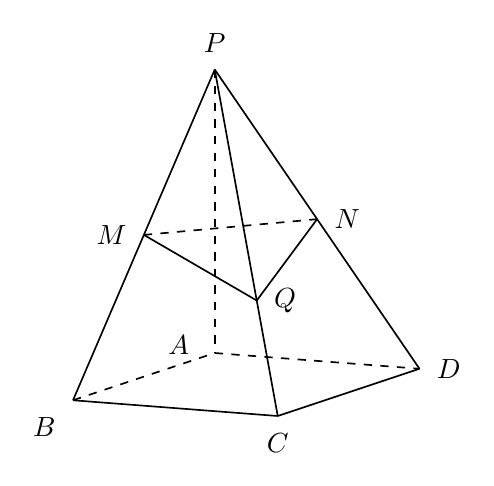
\begin{tikzpicture}[x=1cm,y=1cm,font=\normalsize,line width=.6pt]
\coordinate (P) at (-0.4000000000,4.2000000000);
\coordinate (A) at (-0.4000000000,0.6000000000);
\coordinate (B) at (-2.2,0.0);
\coordinate (C) at (0.4000000000,-0.2000000000);
\coordinate (D) at (2.2,0.4);
\coordinate (M) at (-1.3000000000,2.1000000000);
\coordinate (N) at (0.9000000000,2.3000000000);
\coordinate (Q) at (0.1333333333,1.2666666667);
% solid visible edges
\draw[solid] (P) -- (B);
\draw[solid] (P) -- (D);
\draw[solid] (B) -- (C);
\draw[solid] (C) -- (D);
% hidden edges
\draw[dashed] (P)--(A);
\draw (P)--(C);
\draw[dashed] (M) -- (N);
\draw[dashed] (B) -- (A);
\draw[dashed] (A) -- (D);
\draw (M)--(Q);
\draw (N)--(Q);
% labels with clearance
\node[inner sep=2pt,above=4pt] at (P) {$P$};
\node[inner sep=2pt,left=4pt] at (M) {$M$};
\node[inner sep=2pt,right=4pt] at (N) {$N$};
\node[inner sep=2pt,below left=4pt] at (B) {$B$};
\node[inner sep=2pt,below=4pt] at (C) {$C$};
\node[inner sep=2pt,right=4pt] at (D) {$D$};
\node[inner sep=2pt,left=4pt,xshift=-3pt,yshift=3pt] at (A) {$A$};
\node[inner sep=2pt,right=4pt] at (Q) {$Q$};
\end{tikzpicture}
